\documentclass[cjk,slidestop,compress,mathserif,blue]{beamer}
%dvipdfm选项是关键,否则编译统统通不过
%beamer的颜色选项定义的是导航条和标题的颜色(即关键词structure的颜色)

%%%%%%%%%%%%%%%%仅限于XeTeX可使用的宏包%%%%%%%%%%%%%%%%%%%%%%%%%%%%
\usepackage{fontspec,xunicode,xltxtra,beamerthemesplit}
%\usepackage{beamerthemesplit}
\usepackage{xeCJK}
\setCJKmainfont[BoldFont=黑体, ItalicFont=楷体, BoldItalicFont=仿宋]{黑体}
%\setsansfont[Mapping=tex-text]{Adobe 黑体 Std}
%如果装了Adobe Acrobat,可在font.conf中配置Adobe字体的路径以使用其中文字体
%也可直接使用系统中的中文字体如SimSun,SimHei,微软雅黑 等
%原来beamer用的字体是sans family;注意Mapping的大小写,不能写错

%%%%%%%%   确定标题和导航条结构的框架     %%%%%%%%%%%%
\usepackage{beamerthemeshadow}                       %
%\usepackage{beamerthemeclassic}%导航条色与背景色一致%
%%%%%%%%%%%%%%%%%%%%%%%%%%%%%%%%%%%%%%%%%%%%%%%%%%%%%%
\setbeamerfont{roman title}{size={}}
%\usepackage{CJK} % CJK 中文支持                                  %
\usepackage{amsmath,amsthm,amsfonts,amssymb,bm}
\usepackage{mathrsfs}
\usepackage{xcolor}                                        %使用默认允许使用颜色
\usepackage{hyperref} 
\usepackage{graphicx}
\usepackage{subfigure}           %图片跨页

%\usepackage[numbers,sort&compress]{natbib} %紧密排列             %
\usepackage[sectionbib]{chapterbib}        %每章节单独参考文献   %
\usepackage{hypernat}                                                                         %
%\usepackage[dvipdfm,bookmarksopen=true,pdfstartview=FitH,CJKbookmarks]{hyperref}		%
\hypersetup{bookmarksnumbered,colorlinks,linkcolor=brown,citecolor=blue,urlcolor=red}         %
%参考文献含有超链接引用时需要下列宏包,注意与natbib有冲突        %
%\usepackage[dvipdfm]{hyperref}                                  %
%\usepackage{hypernat}                                           %
\newcommand{\upcite}[1]{\hspace{0ex}\textsuperscript{\cite{#1}}} %

%\useoutertheme{smoothbars}
\useinnertheme[shadow=true]{rounded}
\usetheme{Berkeley}                                          %主题式样
%\usetheme{Luebeck}

\usecolortheme{lily}                                        %颜色主题式样

\usefonttheme{professionalfonts}                           %字体主题样式宏包

%\beamertemplatetransparentcoveredhigh                      %使所有被隐藏的文本高度透明
\beamertemplatetransparentcovereddynamicmedium             %使所有被隐藏的文本完全透明,动态,动态的范围很小
\mode<presentation>
%\beamersetaveragebackground{gray}                          %设置背景颜色(单一色) 
\beamertemplateshadingbackground{green!10}{red!5}         %设置背景颜色(渐变色)

%i放置单位logo
%\logo{\includegraphics[width=1.6cm,height=0.35cm]{Figures/BCC_logo-1.png}}	%简单设置logo

%\pgfdeclareimage[width=3.5cm]{logoname}{Figures/BCC_logo-1.png}		%logo置于左侧微调
%\logo{\pgfuseimage{logoname}{\vspace{0.2cm}\hspace*{-2.0cm}}}

%在指定位置精确放置logo
\usepackage{tikz}
\usepackage{beamerfoils}
\usepackage{pgf}
\logo{\pgfputat{\pgfxy(11.68,0.15)}{\includegraphics[height=1.01cm,viewport=0 0 140 120,clip]{Figures/BCC_logo-1.png}}\pgfputat{\pgfxy(10.502,-0.218)}{\includegraphics[height=0.369cm,viewport=140 0 540 120,clip]{Figures/BCC_logo-1.png}}}
%\logo{\pgfputat{\pgfxy(11.68,0.15)}{\includegraphics[height=0.95cm,viewport=0 0 510 360,clip]{Figures/Logo_Gainstrong.png}}\pgfputat{\pgfxy(10.333,-0.195)}{\includegraphics[height=0.35cm,viewport=530 70 1100 218,clip]{Figures/Logo_Gainstrong.png}}}
%\MyLogo{
%	\pgfputat{\pgfxy(-50,-50)}{\pgfbox[right,base]{\includegraphics[height=1cm]{Figures/BCC_logo-1.png}}}

%logo作为背景放置
%\setbeamertemplate{background}{
%	\pgfputat{\pgfxy(6.5,-0.5)}{\pgfbox[left,top]{\pgfimage[height=1.1cm]{Figures/BCC_logo-1.png}}}}

%\logo{}									%不显示logo

\begin{document}
%\begin{CJK*}{GBK}{song}
%\begin{CJK*}{GBK}{kai}
%beamer下不能用\songyi、\zihao等命令!
%\graphicspath{Figures/}

%-------------------------------PPT Title-------------------------------------
\title{双粒子关联与Bethe-Salpeter方程Bethe-Salpeter方程}
%-----------------------------------------------------------------------------

%----------------------------Author & Date------------------------------------
\author{北京市计算中心\;云平台\:姜骏}
\date{\textrm{2017.01.18}}
%\date{2013.09.10}
\frame{\titlepage}
%-----------------------------------------------------------------------------

%------------------------------------------------------------------------------列出全文 outline ---------------------------------------------------------------------------------
\section*{}
\frame[allowframebreaks]
{
  \frametitle{Outline}
%  \frametitle{\textcolor{mycolor}{\secname}}
  \tableofcontents%[current,currentsection,currentsubsection]
}
%在每个section之前列出全部Outline
%类似的在每个subsection之前列出全部Outline是\AtBeginSubsection[]
\AtBeginSection[]
{
  \frame<handout:0>
  {
    \frametitle{Outline}
%全部Outline中,本部分加亮
    \tableofcontents[current,currentsection]
  }
}

%------------------------------------------------------------------------------PPT main Body------------------------------------------------------------------------------------
\small
\section{扩展体系的线性介电响应}
\frame
{
	\frametitle{独立粒子的极化函数}
	独立粒子在实空间的极化函数(\textcolor{violet}{密度响应函数})定义为
	\begin{displaymath}
		\begin{aligned}
			\chi^0(\vec r,\vec r^{\prime};\omega)=\sum_{\vec k,\vec q}^{\mathrm{BZ}}\sum_{n,n^{\prime}}=&\frac{f_{n,\vec k}-f_{n^{\prime},\vec k+\vec q}}{\omega+\varepsilon_{n,\vec k}-\varepsilon_{n^{\prime},\vec k+\vec q}+\mathrm{i}\eta}\\
			&\times\psi_{n,\vec k}^{\ast}(\vec r)\psi_{n^{\prime},\vec k+\vec q}(\vec r)\psi_{n,\vec k}(\vec r^{\prime})\psi_{n^{\prime},\vec k+\vec q}^{\ast}(\vec r^{\prime})
		\end{aligned}
	\end{displaymath}
	这里$\varepsilon_{n,\vec k}$和$\psi_{n,\vec k}(\vec r)$是波函数的本征态和本征值
	\vskip 5pt
	对占据数$f_{n,\vec k}$的求和满足约束条件
	\begin{displaymath}
		\sum_{n,\vec k}f_{n,\vec k}=N_kN
	\end{displaymath}
	这里$N$数每个原胞的电子数,$N_k$是原胞数目
}

\frame
{
	\frametitle{独立粒子的极化函数}
	对于周期体系,$\chi^0$可用平面波基组展开:
	\begin{displaymath}
		\chi^0(\vec r,\vec r^{\prime};\omega)=\frac1{\Omega}\sum_{\vec q}^{\mathrm{BZ}}\sum_{\vec G\vec G^{\prime}}\mathrm{e}^{\mathrm{i}(\vec q+\vec G)\cdot\vec r}\chi_{\vec G\vec G^{\prime}}^0(\vec q,\omega)\mathrm{e}^{-\mathrm{i}(\vec q+\vec G^{\prime})\cdot\vec r^{\prime}}
	\end{displaymath}
	这里$\vec q$表示入射波的\textrm{Blochl~}矢量,$\vec G(\vec G^{\prime})$是倒格矢
	\vskip 5pt
	再作\textrm{Fourier~}变换可得
	\begin{displaymath}
		\begin{aligned}
			\chi_{\vec G\vec G^{\prime}}^0(\vec q,\omega)=\frac1{\Omega}\sum_{\vec k}^{\mathrm{BZ}}\sum_{n,n^{\prime}}=&\frac{f_{n,\vec k}-f_{n^{\prime},\vec k+\vec q}}{\omega+\varepsilon_{n,\vec k}-\varepsilon_{n^{\prime},\vec k+\vec q}+\mathrm{i}\eta}\\
			&\times\langle\psi_{n,\vec k}|\mathrm{e}^{-\mathrm{i}(\vec q+\vec G)\cdot\vec r}|\psi_{n^{\prime},\vec k+\vec q}\rangle_{\Omega_{\mathrm{cell}}}\\
			&\times\langle\psi_{n,\vec k}|\mathrm{e}^{\mathrm{i}(\vec q+\vec G^{\prime})\cdot\vec r^{\prime}}|\psi_{n^{\prime},\vec k+\vec q}\rangle_{\Omega_{\mathrm{cell}}}
		\end{aligned}
	\end{displaymath}
}

\frame
{
	\frametitle{相互作用体系的极化函数}
	\textcolor{violet}{求解\textrm{Dyson~}方程可得相互作用体系的极化函数}
	\begin{displaymath}
		\chi(\vec r,\vec r^{\prime};\omega)=\chi_0(\vec r,\vec r^{\prime};\omega)+\iint_{\Omega}\mathrm{d}\vec r_1\mathrm{d}\vec r_2\chi_0(\vec r,\vec r_1;\omega)K(\vec r_1,\vec r_2)\chi(\vec r_2,\vec r^{\prime};\omega)
	\end{displaymath}
	这里\textcolor{red}{积分核是所有电子\textrm{Coulomb~}作用和交换-相关作用的求和
		\begin{displaymath}
			K(\vec r_1,\vec r_2)=\frac1{|\vec r_1-\vec r_2|}+\frac{\partial V_{\mathrm{xc}}[n]}{\partial n}
		\end{displaymath}
	}
	类似地,作\textrm{Fourier~}变换,倒空间的\textrm{Dyson~}方程表示为
	\begin{displaymath}
		\chi_{\vec G,\vec G^{\prime}}(\vec q,\omega)=\chi_{\vec G,\vec G^{\prime}}^0(\vec q,\omega)+\sum_{\vec G_1\vec G_2}\chi_{\vec G\vec G_1}^0(\vec q,\omega)K_{\vec G_1\vec G_2}(\vec q)\chi_{\vec G_2\vec G^{\prime}}(\vec q,\omega)
	\end{displaymath}
	\textcolor{red}{注意}:~\textcolor{blue}{倒空间中电子的\textrm{Coulomb~}作用对积分核$K$的贡献
	\begin{displaymath}
		K_{\vec G_1\vec G_2}^{\mathrm{Coulomb}}(\vec q)=\frac{4\pi}{\vec q+\vec G_1}\delta_{\vec G_1\vec G_2}
	\end{displaymath}}
}

\frame
{
	\frametitle{相互作用体系的极化函数}
	\textcolor{violet}{倒空间中交换-相关的贡献由\textrm{adiabatic local density approximation (ALDA)}~计算
	\begin{displaymath}
		K_{\vec G_1\vec G_2}^{\mathrm{xc,ALDA}}(\vec q)=\frac1{\Omega}\int\mathrm{d}\vec rf_{\mathrm{xc}}[n(\vec r)]\mathrm{e}^{-\mathrm{i}(\vec G_1-\vec G_2)\cdot\vec r}
	\end{displaymath}}
	这里
	\begin{displaymath}
		f_{\mathrm{xc}}[n(\vec r)]=\left.\frac{\partial^2E_{\mathrm{xc}}[n]}{\partial n^2}\right|_{n_0(\vec r)}
	\end{displaymath}
}

\frame
{
	\frametitle{介电函数和有关谱函数}
	介电函数矩阵用极化矩阵表示
	\begin{displaymath}
		\epsilon_{\vec G\vec G^{\prime}}^{-1}(\vec q,\omega)=\delta_{\vec G\vec G^{\prime}}+\frac{4\pi}{|\vec q+\vec G|^2}\chi_{\vec G\vec G^{\prime}}(\vec q,\omega)
	\end{displaymath}
	\textrm{RPA~}近似下,介电函数矩阵可以表示为
	\begin{displaymath}
		\epsilon_{\vec G\vec G^{\prime}}^{\textcolor{red}{\mathrm{RPA}}}(\vec q,\omega)=\delta_{\vec G\vec G^{\prime}}-\frac{4\pi}{|\vec q+\vec G|^2}\chi_{\vec G\vec G^{\prime}}^0(\vec q,\omega)
	\end{displaymath}
	\textcolor{red}{宏观介电函数}(更严格的记作$\epsilon_M^{\textcolor{red}{LF}}(\vec q,\omega)$)的定义
	\begin{displaymath}
		\epsilon_M(\vec q,\omega)=\frac1{\epsilon_{00}^{\textcolor{red}{-1}}(\vec q,\omega)}
	\end{displaymath}
	光学吸收函数
	\begin{displaymath}
		\mathrm{ABS}=\mathrm{Im}\epsilon_M(\vec q\rightarrow0,\omega)
	\end{displaymath}
	电子能量损失函数(\textrm{electron energy loss spectrum, EELS})
	\begin{displaymath}
		\mathrm{EELS}=-\mathrm{Im}\frac1{\epsilon_M(\vec q,\omega)}
	\end{displaymath}
}

\frame
{
	\frametitle{\textrm{Hilbert~}变换}
	通过\textrm{Hilbert~}变换,独立粒子极化函数$\chi_{\vec G\vec G^{\prime}}^0(\vec q,\omega)$可用谱函数表示
	\begin{displaymath}
		\chi_{\vec G\vec G^{\prime}}^0(\vec q,\omega)=\int_{-\infty}^{+\infty}\mathrm{d}\omega^{\prime}\frac{A_{\vec G\vec G^{\prime}}(\vec q,\omega^{\prime})}{\omega-\omega^{\prime}+\mathrm{i}\eta}
	\end{displaymath}
	这里谱函数$A_{\vec G\vec G^{\prime}}(\vec q,\omega^{\prime})$定义为
	\begin{displaymath}
		\begin{aligned}
			A_{\vec G\vec G^{\prime}}(\vec q,\omega^{\prime})&=\frac1{\Omega}\sum_{\vec k}^{\mathrm{BZ}}\sum_{n,n^{\prime}}(f_{n,\vec k}-f_{n^{\prime},\vec k+\vec q})\langle\psi_{n,\vec k}|\mathrm{e}^{-\mathrm{i}(\vec q+\vec G)\cdot\vec r}|\psi_{n^{\prime},\vec k+\vec q}\rangle\\
			&\times\langle\psi_{n,\vec k}|\mathrm{e}^{\mathrm{i}(\vec q+\vec G^{\prime})\cdot\vec r^{\prime}}|\psi_{n^{\prime},\vec k+\vec q}\rangle\times\delta(\omega^{\prime}+\varepsilon_{n,\vec k}-\varepsilon_{n^{\prime},\vec k+\vec q})
		\end{aligned}
	\end{displaymath}
	\textcolor{red}{注意}:~上述积分范围包含\textcolor{blue}{“正”}和\textcolor{blue}{“负”}两部分频率
	\vskip 5pt
	对于包含时间反演对称性的体系,本征态满足
	\begin{displaymath}
		\varepsilon_{n,-\vec k}=\varepsilon_{n,\vec k}\quad f_{n,-\vec k}=f_{n,\vec k}\quad\psi_{n,-\vec k}(\vec r)=\psi_{n,\vec k}^{\ast}(\vec r)
	\end{displaymath}
}

\frame
{
	\frametitle{\textrm{Hilbert~}变换}
	变换谱函数$A_{\vec G\vec G^{\prime}}(\vec q,\omega^{\prime})$指标
	\begin{displaymath}
		\begin{aligned}
			&n,\vec k\rightarrow n^{\prime},-\vec k-\vec q\\
			&n^{\prime},\vec k+\vec q\rightarrow n,-\vec k
		\end{aligned}
	\end{displaymath}
	利用时间反演对称性
	\begin{displaymath}
		A_{\vec G\vec G^{\prime}}(\vec q,\omega^{\prime})=-A_{\vec G\vec G^{\prime}}(\vec q,-\omega^{\prime})
	\end{displaymath}
	因此可有
	\begin{displaymath}
		\begin{aligned}
			\chi_{\vec G\vec G^{\prime}}^0(\vec q,\omega)=&\int_{-\infty}^0\mathrm{d}\omega^{\prime}\frac{A_{\vec G\vec G^{\prime}}(\vec q,\omega^{\prime})}{\omega-\omega^{\prime}+\mathrm{i}\eta}+\int_0^{+\infty}\mathrm{d}\omega^{\prime}\frac{A_{\vec G\vec G^{\prime}}(\vec q,\omega^{\prime})}{\omega-\omega^{\prime}+\mathrm{i}\eta}\\
			=&\int_0^{+\infty}\mathrm{d}\omega^{\prime}\left[ \frac1{\omega-\omega^{\prime}+\mathrm{i}\eta}-\frac1{\omega+\omega^{\prime}+\mathrm{i}\eta} \right]A_{\vec G\vec G^{\prime}}(\vec q,\omega^{\prime})
		\end{aligned}
	\end{displaymath}
}

\section{\rm{Bethe-Salpeter~}方程}
\frame
{
	\frametitle{\textrm{GWA~}的问题}
	在\textrm{Kohn-Sham~}方程的本征态基础上,\textcolor{purple}{用\textrm{RPA~}计算极化函数,由于顶角函数过于简单},计算光学性质与实验结果往往出现不一致
	\begin{itemize}
		\item 光学吸收谱函数与实验结果出现定量或定性不符
		\item 准粒子(\textrm{GWA~}校正)本征态能量计算的带隙与实验结果不符
	\end{itemize}
\begin{figure}[h!]
\centering
\vspace*{-0.12in}
\includegraphics[height=1.6in,width=2.7in,viewport=0 0 1000 600,clip]{Figures/BSE_GW_DFT.png}
\caption{\small \textrm{Schematic picture of the different levels of the description of optical spectra available in DFT, GW, BSE.}}%
\label{DFT_GW_BSE}
\end{figure} 
}

\frame
{
	\frametitle{\textrm{Bethe-Salpeter~}方程}
	\begin{itemize}
		\item 在凝聚态物理中,绝缘体和半导体的光谱容易受到电子-空穴相互作用的影响(\textcolor{red}{\textrm{RPA~}完全忽略了电子-空穴相互作用}),为了正确考虑电子-空穴的相互作用,可以通过\textrm{Bethe-Salpeter~}方程计算双粒子的关联函数(\textrm{Correlation Function})$L$得到
		\item \textrm{Bethe-Salpeter~}方程描述的是双体束缚态相对论运动,在多体理论(\textrm{Many-body Theory})中,\textrm{Bethe-Salpeter~}方程用\textrm{Feynman Diagram~}可表示为
\begin{figure}[h!]
\centering
\vspace*{-0.1in}
\includegraphics[height=0.9in,width=2.1in,viewport=0 0 650 280,clip]{Figures/BSE_Feynman.png}
\caption{\small \textrm{Feynman diagrams representing the four point Bethe-Salpeter equation}}%
\label{BSE_Feynman}
\end{figure} 
	\end{itemize}
}

\frame
{
	\frametitle{\textrm{Bethe-Salpeter~}方程}
	\begin{itemize}
		\item \textrm{Bethe-Salpeter~}方程
\begin{figure}[h!]
\centering
\vspace*{-0.15in}
\includegraphics[height=0.5in,width=2.6in,viewport=0 0 350 65,clip]{Figures/BS_equation.png}
%\caption{\small \textrm{Feynman diagrams representing the four point Bethe-Salpeter equation}}%
\label{BS_equation-1}
\end{figure} 
\begin{displaymath}
	\textcolor{red}{L=GG+GG\Xi L}
\end{displaymath}
		\item \textrm{Interaction Kernel~}方程
\begin{figure}[h!]
\centering
%\vspace*{-0.1in}
\includegraphics[height=0.5in,width=2.0in,viewport=0 0 250 65,clip]{Figures/K_equation.png}
%\caption{\small \textrm{Feynman diagrams representing the four point Bethe-Salpeter equation}}%
\label{BS_equation-2}
\end{figure} 
\begin{displaymath}
	\textcolor{blue}{\Xi=\frac{\delta\Sigma}{\delta G}\cong-\mathrm{i}v+\mathrm{i}W}
\end{displaymath}
	\end{itemize}
}

\frame
{
	\frametitle{\textrm{Bethe-Salpeter~}方程的函数定义}
\begin{itemize}
	\item 双粒子关联函数$L$
		\begin{displaymath}
			L(\mathbf{1},\mathbf{2},\mathbf{3},\mathbf{4})=-G^{(2)}(\mathbf{1},\mathbf{2},\mathbf{3},\mathbf{4})+G(\mathbf{1},\mathbf{3})G(\mathbf{2},\mathbf{4})
		\end{displaymath}
		这里$G^{(2)}(\mathbf{1},\mathbf{2},\mathbf{3},\mathbf{4})$是双粒子\textrm{Green's function}
		\vskip 5pt
		这里$G(\mathbf{1},\mathbf{2})$是单粒子\textrm{Green's function}

	\item 极化函数
		\begin{displaymath}
			\chi(\mathrm{1},\mathbf{2})=-\mathrm{i}L(\mathbf{1},\mathbf{2},\mathbf{1}^+,\mathbf{2}^+)
		\end{displaymath}
	\item 宏观介电函数
		\begin{displaymath}
			\epsilon(\omega)=1-v\chi(\omega)
		\end{displaymath}
\end{itemize}
}

\frame
{
	\frametitle{\textrm{Bethe-Salpeter~}方程}
\textrm{Bethe-Salpeter~}方程也可以写为
\begin{displaymath}
	\hspace*{-10pt}
	\begin{aligned}
		&\chi(\vec r_1,\vec r_2,\vec r_3,\vec r_4;\omega)=\chi^0(\vec r_1,\vec r_2,\vec r_3,\vec r_4;\omega)\\
		+&\int\mathrm{d}\vec r_5\mathrm{d}\vec r_6\mathrm{d}\vec r_7\mathrm{d}\vec r_8\chi^0(\vec r_1,\vec r_2,\vec r_5,\vec r_6;\omega)K(\vec r_5,\vec r_6,\vec r_7,\vec r_8;\omega)\chi(\vec r_7,\vec r_8,\vec r_3,\vec r_4;\omega)
	\end{aligned}
\end{displaymath}
这里
\begin{displaymath}
	K=v-W=\frac1{|\vec r_5-\vec r_7|}\delta_{\vec r_5,\vec r_6}\delta_{\vec r_7,\vec r_8}-\int\mathrm{d}\vec r\frac{\epsilon^{-1}(\vec r_5,\vec r;\omega)}{|\vec r-\vec r_6|}\delta_{\vec r_5,\vec r_7}\delta_{\vec r_6,\vec r_8}
\end{displaymath}
注意到极化函数$\chi(\vec r,\vec r^{\prime})=\delta n(\vec r)/\delta V_{ext}(\vec r^{\prime})$,有
\begin{displaymath}
	\chi(\vec r_1,\vec r_2,\vec r_3,\vec r_4;\omega)=\chi(\vec r_1,\vec r_3;\omega)\delta_{\vec r_1,\vec r_2}\delta_{\vec r_3,\vec r_4}
\end{displaymath}
\textrm{Bethe-Salpeter~}方程可简化为
\begin{displaymath}
	\begin{aligned}
		\chi(\vec r,\vec r^{\prime};\omega)=\chi^0(\vec r,\vec r^{\prime};\omega)+\int\mathrm{d}\vec r_5\mathrm{d}\vec r_7\chi^0(\vec r,\vec r_5;\omega)\frac1{|\vec r_5-\vec r_7|}\chi(\vec r_7,\vec r^{\prime};\omega)\\
		+\int\mathrm{d}\vec r_5\mathrm{d}\vec r_6\mathrm{d}r^{\prime\prime}\chi^0(\vec r,\vec r_5,\vec r_6;\omega)\frac{\epsilon^{-1}(\vec r_5,\vec r^{\prime\prime};\omega)}{|\vec r^{\prime\prime}-\vec r_6|}\chi(\vec r_5,\vec r_6,\vec r^{\prime};\omega)
	\end{aligned}
\end{displaymath}
}

\frame
{
	\frametitle{\textrm{Bethe-Salpeter~}方程的求解流程}
\begin{figure}[h!]
\centering
\vspace*{-0.26in}
\includegraphics[height=3.07in,width=1.65in,viewport=0 0 380 850,clip]{Figures/BSE_flow.png}
\caption{\small \textrm{Flow diagram sketching the solution of the Bethe-Salpeter equation}}%
\label{BS_equation-1}
\end{figure} 
}

\frame
{
	\frametitle{电子-空穴对基变换}
	假设\textrm{Kohn-Sham~}方程的本征态构成正交完备基组,任意四点函数(双粒子函数)$S$可以用“对波函数”变换
	\begin{displaymath}
		S(\vec r_1,\vec r_2,\vec r_3,\vec r_4;\omega)=\sum_{n_1,n_2,n_3,n_4}\psi_{n_1}^{\ast}(\vec r_1)\psi_{n_2}(\vec r_2)\psi_{n_3}(\vec r_3)\psi_{n_4}^{\ast}(\vec r_4)S_{\substack{n_1 n_2\\n_3 n_4 }}(\omega)
	\end{displaymath}
	类似地,无相互作用极化函数$\chi^0$
	\begin{displaymath}
		\chi^0(\vec r_1,\vec r_2,\vec r_3,\vec r_4;\omega)=\sum_{nn^{\prime}}\frac{f_n-f_{n^{\prime}}}{\varepsilon_n-\varepsilon_{n^{\prime}}-\omega}\psi_n^{\ast}(\vec r_1)\psi_{n^{\prime}}(\vec r_2)\psi_n(\vec r_3)\psi_{n^{\prime}}^{\ast}(\vec r_4)
	\end{displaymath}
用“对函数”表示
\begin{displaymath}
	\chi_{ \substack {n_1 n_2\\n_3 n_4}  }^0
		(\omega)=\frac{f_{n_2}-f_{n_1}}{\varepsilon_{n_2}-\varepsilon_{n_1}-\omega}\delta_{n_1n_3}\delta_{n_2n_4}
\end{displaymath}
}

\frame
{
	\frametitle{电子-空穴对基变换}
	四点\textrm{Bethe-Salpeter~}方程在“对函数”空间表示
	\begin{displaymath}
		\chi_{ \substack{ n_1 n_2\\n_3 n_4 } }
		(\omega)=\chi_{n_1n_2}^0(\omega)\left[ \delta_{n_1n_3}\delta_{n_2n_4}+\sum_{n_5n_6}K_{
			\substack{	n_1 n_2\\ n_5 n_6 } }
			(\omega)\chi_{
				\substack{ n_5 n_6\\ n_3 n_4 } }(\omega)
			\right]
	\end{displaymath}
	由$K=v-W$可有
	\begin{displaymath}
		v_{
			\substack{ n_1 n_2\\ n_5 n_6 } }
			=\int\mathrm{d}\vec r\mathrm{d}\vec r^{\prime}\psi_{n_1}(\vec r)\psi_{n_2}^{\ast}(\vec r)\frac1{|\vec r-\vec r^{\prime}|}\psi_{n_5}^{\ast}(\vec r^{\prime})\psi_{n_6}(\vec r^{\prime})
	\end{displaymath}
	\begin{displaymath}
		W_{
			\substack{
				n_1 n_2\\
				n_5 n_6
			} }=\int\mathrm{d}\vec r\mathrm{d}\vec r^{\prime}\mathrm{d}\vec r^{\prime\prime}\psi_{n_1}(\vec r)\psi_{n_2}^{\ast}(\vec r^{\prime})\frac{\epsilon^{-1}(\vec r,\vec r^{\prime\prime};\omega)}{|\vec r^{\prime\prime}-\vec r^{\prime}|}\psi_{n_5}^{\ast}(\vec r)\psi_{n_6}(\vec r^{\prime})
	\end{displaymath}
}

\frame
{
	\frametitle{\textrm{Bethe-Salpeter~}方程变换为有效双粒子\textrm{Hamiltonian}}
	为求解\textrm{Bethe-Salpeter~}方程,对每个频率作矩阵求逆,可将问题转化为本征值问题
	\begin{displaymath}
		\sum_{n_5n_6}\left[ \delta_{n_1n_5}\delta_{n_2n_6}-\chi_{n_1n_2}^0(\omega)K_{
			\substack{
				n_1 n_2\\
				n_5 n_6
			} }
			(\omega)
			\right]\chi_{ \substack{
			n_5 n_6\\n_3 n_4 
		} }
		(\omega)=\chi_{n_1n_2}^0(\omega)
	\end{displaymath}
	\vskip 20pt
	化简得
	\begin{displaymath}
		\begin{aligned}
			&\sum_{n_5n_6}\left[ (\varepsilon_{n_1}-\varepsilon_{n_2}-\omega)\delta_{n_1n_5}\delta_{n_2n_6}-(f_{n_2}-f_{n_1})K_{
			\substack{
				n_1 n_2\\
				n_5 n_6
			} }
			(\omega)
			\right]\chi_{ \substack{
			n_5 n_6\\n_3 n_4 
		} }
		(\omega)\\
		=&f_{n_2}-f_{n_1}
		\end{aligned}
	\end{displaymath}
}

\frame
{
	\frametitle{\textrm{Bethe-Salpeter~}方程变换为有效双粒子\textrm{Hamiltonian}}
	考虑静电相互作用的积分核$K(\omega=0)$函数,可定义有效双粒子\textrm{Hamiltonian~}为
	\begin{displaymath}
		\mathcal{H}_{
			\substack{
				n_1 n_2\\
				n_5 n_6
			} }\equiv(\varepsilon_{n_2}-\varepsilon_{n_1})\delta_{n_1n_5}\delta_{n_2n_6}-(f_{n_2}-f_{n_1})K_{
			\substack{
				n_1 n_2\\
				n_5 n_6
			} }
	\end{displaymath}
	因此对应的\textrm{Bethe-Salpeter~}方程可写成
	\begin{displaymath}
		\chi_{ \substack{
			n_1 n_2\\n_3 n_4 
		} }=[\mathcal{H}-\mathcal{I}\omega]_{
			\substack{
				n_1 n_2\\
				n_3 n_4
			} }^{-1}(f_{n_2}-f_{n_1})
		\end{displaymath}
		这里$\mathcal{I}$是与$\mathcal{H}$有相同维度的单位矩阵
\vskip 5pt
\textcolor{violet}{对角化\textrm{Hamiltonian~}$\mathcal{H}$,得到的能量本征值是元激发的激发能,激发强度可由本征矢表示}
}

\frame
{
	\frametitle{\textrm{Bethe-Salpeter~}方程变换为有效双粒子\textrm{Hamiltonian}}
	谱表示的双粒子\textrm{Hamiltonian~}逆可写成
	\begin{displaymath}
		[\mathcal{H}-\mathcal{I}\omega]_{
			\substack{
				n_1 n_2\\
				n_3 n_4
			} }^{-1}=\sum_{\lambda,\lambda^{\prime}}\frac{A_{\lambda}^{n_1n_2}A_{\lambda^{\prime}}^{n_3n_4}N_{\lambda\lambda^{\prime}}^{-1}}{E_{\lambda}-\omega}
	\end{displaymath}
	这里本征值$E_{\lambda}$和本征矢$A_{\lambda}$满足
	\begin{displaymath}
		\mathcal{H}A_{\lambda}=E_{\lambda}A_{\lambda}
	\end{displaymath}
	重叠矩阵$N_{\lambda\lambda^{\prime}}$定义为
	\begin{displaymath}
		N_{\lambda\lambda^{\prime}}\equiv\sum_{n_1n_2}[A_{\lambda}^{n_1n_2}]^{\ast}A_{\lambda^{\prime}}^{n_1n_2}
	\end{displaymath}
	如果\textrm{Hamiltonian~}$\mathcal{H}$是\textrm{Hermitian},本征矢$A_{\lambda}$是正交的,并有
	\begin{displaymath}
		N_{\lambda\lambda^{\prime}}=\delta_{\lambda\lambda^{\prime}}
	\end{displaymath}
}

\frame
{
	\frametitle{方程在$\vec k$空间的依赖关系}
	双粒子\textrm{Hamiltonian~}的倒空间表示
	\fontsize{8.5pt}{6.2pt}\selectfont{\begin{displaymath}
		\hspace*{-10pt}
		\mathcal{H}_{
			\substack{
				n_1 n_2 \vec k_1\\
				n_5 n_6 \vec k_5
			} }(\vec q)\equiv(\varepsilon_{n_2,\vec k_1+\vec q}-\varepsilon_{n_1,\vec k_1})\delta_{n_1n_5}\delta_{n_2n_6}\delta_{\vec k_1\vec k_5}-(f_{n_2,\vec k_1+\vec q}-f_{n_1,\vec k_1})K_{
			\substack{
				n_1 n_2 \vec k_1\\
				n_5 n_6 \vec k_5
			} }(\vec q)
		\end{displaymath}}
		相应的$K=v-W$可表示为
	\fontsize{8.5pt}{6.2pt}\selectfont{\begin{displaymath}
		\hspace*{-10pt}
		v_{
			\substack{
				n_1 n_2 \vec k_1\\
				n_5 n_6 \vec k_5
			} }(\vec q)=\int\mathrm{d}\vec r\mathrm{d}\vec r^{\prime}\psi_{n_1,\vec k_1}(\vec r)\psi_{n_2,\vec k_1+\vec q}^{\ast}(\vec r)\frac1{|\vec r-\vec r^{\prime}|}\psi_{n_5,\vec k_5}^{\ast}(\vec r^{\prime})\psi_{n_6,\vec k_1+\vec q}(\vec r^{\prime})
		\end{displaymath}}
	\fontsize{8.5pt}{6.2pt}\selectfont{\begin{displaymath}
		\hspace*{-10pt}
		W_{
			\substack{
				n_1 n_2 \vec k_1\\
				n_5 n_6 \vec k_2
			} }(\vec q)=\int\mathrm{d}\vec r\mathrm{d}\vec r^{\prime}\psi_{n_1,\vec k_1}(\vec r)\psi_{n_2,\vec k_1+\vec q}^{\ast}(\vec r^{\prime})\frac{\epsilon^{-1}(\vec r,\vec r^{\prime};\omega=0)}{|\vec r-\vec r^{\prime}|}\psi_{n_5,\vec k_5}^{\ast}(\vec r)\psi_{n_6,\vec k_5+\vec q}(\vec r^{\prime})
		\end{displaymath}}
		“对函数”空间表示下极化函数表示为
		\begin{displaymath}
			\chi_{
				\substack{
					n_1 n_2 \vec k_1\\
					n_3 n_4 \vec k_3
				} }(\vec q,\omega)=\sum_{\lambda\lambda^{\prime}}\frac{A_{\lambda}^{n_1n_2,\vec k_1}A_{\lambda^{\prime}}^{n_3n_4,\vec k_3}N_{\lambda\lambda^{\prime}}^{-1}}{E_{\lambda}-\omega}(f_{n_2,\vec k_1+\vec q}-f_{n_1,\vec k_1})
		\end{displaymath}
}

\frame
{
	\frametitle{“对函数”空间与倒空间表示的变换}
	根据长波极限下,标量介电函数与极化函数的关系
	\begin{displaymath}
		\chi_{\vec G\vec G^{\prime}}(\vec q,\omega)=\frac1{\Omega}\sum_{\substack{n_1n_2,\vec k_1\\n_3n_4,\vec k_3}}\chi_{\substack{n_1n_2,\vec k_1\\n_3n_4,\vec k_3}}(\vec q,\omega)\rho_{\substack{n_1,\vec k_1\\n_2,\vec k_1+\vec q}}(\vec G)\rho_{\substack{n_3,\vec k_3\\n_4,\vec k_3+\vec q}}^{\ast}(\vec G^{\prime})
	\end{displaymath}
这里密度矩阵$\rho(\vec G)$的定义为
\begin{displaymath}
	\rho_{\substack{n_1,\vec k_1\\n_2,\vec k_1+\vec q}}\equiv\langle\psi_{n_1,\vec k_1}|\mathrm{e}^{-\mathrm{i}(\vec q+\vec G)\cdot\vec r}|\psi_{n_2,\vec k_1+\vec q}\rangle
\end{displaymath}
由\textrm{Fourier~}变换
\begin{displaymath}
	\begin{aligned}
		\frac1{|\vec r-\vec r^{\prime}|}=&\frac1{\Omega}\sum_{\vec q\vec G}\frac{4\pi}{|\vec q+\vec G|^2}\mathrm{e}^{\mathrm{i}(\vec q+\vec G)\cdot(\vec r-\vec r^{\prime})}\\
		\int\mathrm{d}\vec r^{\prime\prime}\frac{\epsilon^{-1}(\vec r,\vec r^{\prime\prime})}{|\vec r^{\prime\prime}-\vec r^{\prime}|}=&\frac1{\Omega}\sum_{\vec q\vec G\vec G^{\prime}}\mathrm{e}^{\mathrm{i}(\vec q+\vec G)\cdot\vec r}\frac{4\pi\epsilon_{\vec G\vec G^{\prime}}^{-1}(\vec q)}{|\vec q+\vec G|^2}\mathrm{e}^{-\mathrm{i}(\vec q+\vec G^{\prime})\cdot\vec r^{\prime}}
	\end{aligned}
\end{displaymath}
}

\frame
{
	\frametitle{“对函数”空间与倒空间表示的变换}
	\begin{displaymath}
		\begin{aligned}
			v_{\substack{n_1n_2,\vec k_1\\n_5n_6,\vec k_5}}=&\sum_{\vec G}\rho_{\substack{n_1,\vec k_1\\n_2,\vec k_1+\vec q}}^{\ast}(\vec G)\frac{4\pi}{|\vec q+\vec G|^2\rho_{\substack{n_5,\vec k_5\\n_6,\vec k_5+\vec q}}(\vec G)}\\
			W_{\substack{n_1n_2,\vec k_1\\n_5n_6,\vec k_5}}=&\sum_{\vec G\vec G^{\prime}}\rho_{\substack{n_1,\vec k_1\\n_5,\vec k_5}}^{\ast}(\vec G)\frac{4\pi\epsilon_{\vec G\vec G^{\prime}}^{-1}(\vec q;\omega=0)}{|\vec q+\vec G|^2\rho_{\substack{n_2,\vec k_1+\vec q\\n_6,\vec k_5+\vec q}}(\vec G^{\prime})}
		\end{aligned}
	\end{displaymath}

	已知介电函数矩阵与极化函数关系
	\begin{displaymath}
		\epsilon_{\vec G\vec G^{\prime}}^{-1}(\vec q,\omega)=\delta_{\vec G\vec G^{\prime}}+\frac{4\pi}{|\vec q+\vec G|^2}\chi_{\vec G\vec G^{\prime}}(\vec q,\omega)
	\end{displaymath}
	能量损失函数(\textrm{EELS})正比于$-\mathrm{Im}\epsilon_{00}^{-1}$
	\begin{displaymath}
		\mathrm{EELS}\propto-\mathrm{Im}\epsilon_{00}^{-1}(\vec q,\omega)=-\frac{4\pi}{|\vec q|^2}\mathrm{Im}\chi_{00}(\vec q,\omega)
	\end{displaymath}
}

\frame
{
	\frametitle{介电函数和光谱函数}
	长波极限下,宏观吸收光谱\textrm{ABS}由函数$\mathrm{Im}\epsilon_M$计算,直接通过计算$\epsilon_{00}^{-1}$获得,比较麻烦,可通过极化函数$\bar\chi$计算
	\begin{displaymath}
		\begin{aligned}
			\epsilon_M(\omega)=&1-\frac{4\pi}{|\vec q|^2}\bar{\chi}_{00}(\vec q\rightarrow0,\omega)\\
			\mathrm{ABS}=\mathrm{Im}\epsilon_M(\omega)=&-\frac{4\pi}{|\vec q|^2}\bar{\chi}_{00}(\vec q\rightarrow0,\omega)
		\end{aligned}
	\end{displaymath}
	相应的极化函数$\bar{\chi}$与原始的$\chi$的计算方案相同,只是不考虑\textrm{Coulomb~}项贡献
	\begin{displaymath}
		\bar{v}_{\substack{n_1n_2,\vec k_1\\n_5n_6,\vec k_5}}(\vec q)=\sum_{\vec G\neq0}\rho_{\substack{n_1,\vec k_1\\n_2,\vec k_1+\vec q}}^{\ast}(\vec G)\frac{4\pi}{|\vec q+\vec G|^2}\rho_{\substack{n_5,\vec k_5\\n_6,\vec k_5+\vec q}}(\vec G)
	\end{displaymath}
}

%\frame
%{
%\frametitle{发展统一理论框架下的材料计算程序}
%\begin{itemize}
%	\item
%\end{itemize}
%}

%\appendix
%------------------------------------------------------------------------Reference----------------------------------------------------------------------------------------------
%\begin{thebibliography}{99}
%-----------------------------------------------------------------------------------------------------------------------------------------------------------------------%
%\frame
%{
%\frametitle{主要参考文献}
%{\small
%\bibitem{Singh_Book}\textrm{D. J. Singh. \textit{Plane Wave, PseudoPotential and the LAPW method} (Kluwer Academic, Boston,USA, 1994)}					%
%  \nocite{*}																				%
%}
%}
%\end{thebibliography}
\begin{thebibliography}{99}
\frame
{
\frametitle{主要参考文献}
{\small
%	\bibitem{Huang_Han}黄昆\:原著、韩汝琦\:改编, {\textit{固体物理学}}\:高等教育出版社, 北京, 1988
%	\bibitem{Xie_Lu}谢希德、陆栋\:主编, {\textit{固体能带理论}}\:复旦大学出版社, 上海, 1998
        \bibitem{Inkson_Book}\textrm{J. C. Inkson. \textit{Many-Body Theory of Solids: An Introduction} (Plenum Press, New York, USA, 1984)}
	\bibitem{Bruus_Flensberg}\textrm{H. Bruus and K. Flensberg. \textit{Many-Body Quantum Theory in Condensed Matter Physics: An Introduction} (Oxford University Press, U.K., 2004)}
	\bibitem{PR84-1232_1951}\textrm{E. E. Salpeeter and H. A. Bethe \textit{Phys. Rev.}, \textbf{84} (1951), 1232}
	\bibitem{PR139-A796_1965}\textrm{L. Hedin. \textit{Phys. Rev.}, \textbf{139} (1965), A796}
	\bibitem{RMP74-601_2002}\fontsize{9.6pt}{3.9pt}\selectfont{\textcolor{red}{\frame{\textrm{G. Onida, L. Reining and A. Rubio. \textit{Rev. Mod. Phys.}, \textbf{74} (2002), 601}}}}
	\bibitem{CPC20-11_1980}\textrm{R. Haydock. \textit{Comput. Phys. Comm.}, \textbf{20} (1980), 11}
	\bibitem{NL9-2820_2009}\textrm{M. Gruning, A. Marini and X. Gonze. \textit{Nano. Lett.}, \textbf{9} (2009), 2820}
	\bibitem{PRB33-7017_1986}\textrm{S. Baroni and R. Resta. \textit{Phys. Rev. B}, \textbf{33} (1986), 7017}
}
\nocite*{}
}
\end{thebibliography}
%{\small
%\phantomsection\addcontentsline{toc}{section}{Bibliography}	 %直接调用\addcontentsline命令可能导致超链指向不准确,一般需要在之前调用一次\phantomsection命令加以修正	%
%\bibliography{Myref}																			%
%\bibliographystyle{mybib}																		%
%  \nocite{*}																				%
%}
%-----------------------------------------------------------------------------------------------------------------------------------------------------------------------%


%-----------------------------------------------------------Beamer下不建议使用bib,因为涉及分页--------------------------------------------------------------------------%
%{\small
%\phantomsection\addcontentsline{toc}{section}{Bibliography}	 %直接调用\addcontentsline命令可能导致超链指向不准确,一般需要在之前调用一次\phantomsection命令加以修正	%
%\bibliography{Myref}																			%
%\bibliographystyle{mybib}																		%
%  \nocite{*}																				%
%}

%------------------------------------------------------------------------------------------------------------------------------------------------------------------------------%

\appendix
\section{VASP的主程序}
\frame
{
\frametitle{}
\begin{figure}[h!]
\centering
\vspace*{-0.80in}
%\hspace*{-10pt}
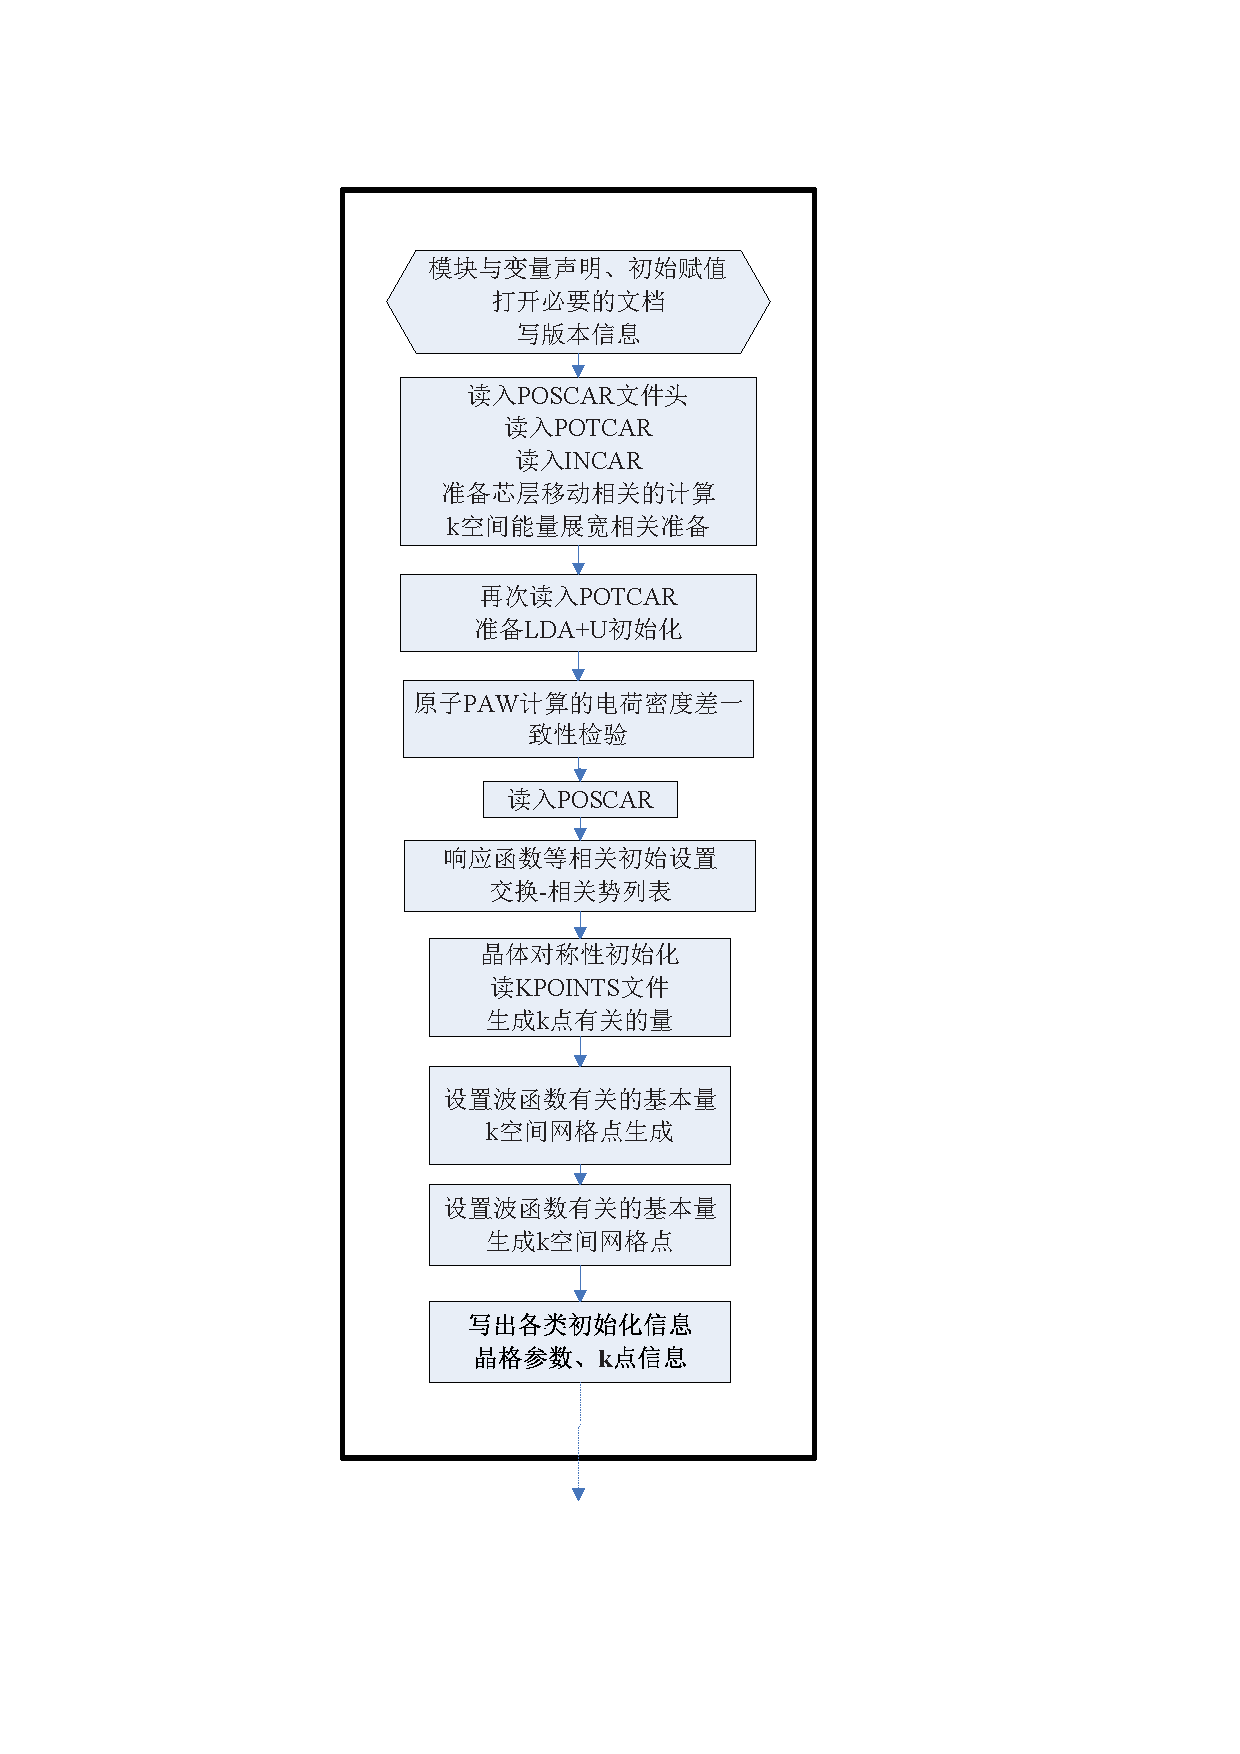
\includegraphics[height=3.72in,width=2.5in,viewport=160 118 395 755,clip]{Figures/VASP_main_Flow-1.pdf}
\caption{\small \textrm{Calculation of the K-S ground-states.}}%
\label{VASP_Follow-1}
\end{figure}
}

\frame
{
\frametitle{}
\begin{figure}[h!]
\centering
\vspace*{-0.80in}
%\hspace*{-10pt}
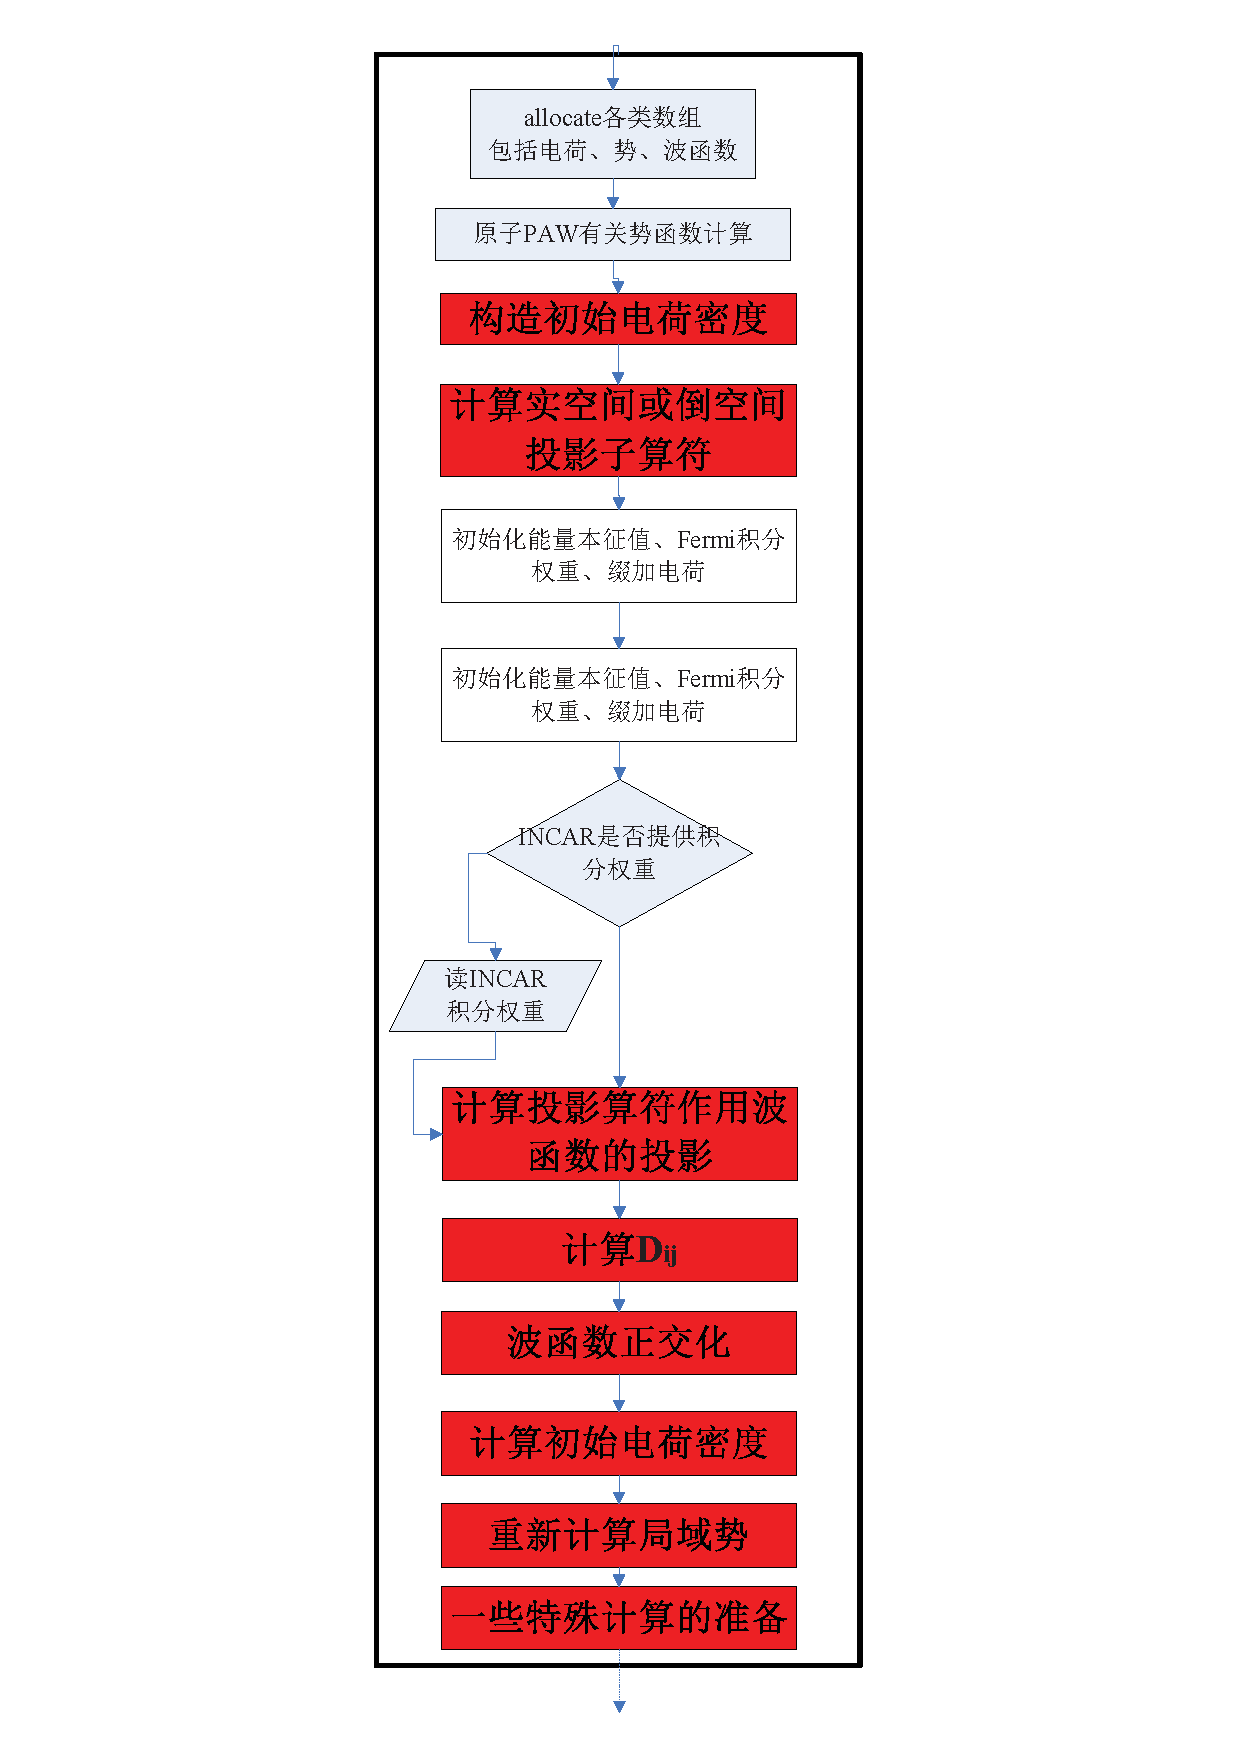
\includegraphics[height=3.72in,width=2.5in,viewport=170 16 416 819,clip]{Figures/VASP_main_Flow-2.pdf}
\caption{\small \textrm{Calculation of the K-S ground-states.}}%
\label{VASP_Follow-2}
\end{figure}
}

\frame
{
\frametitle{}
\begin{figure}[h!]
\centering
\vspace*{-0.80in}
%\hspace*{-10pt}
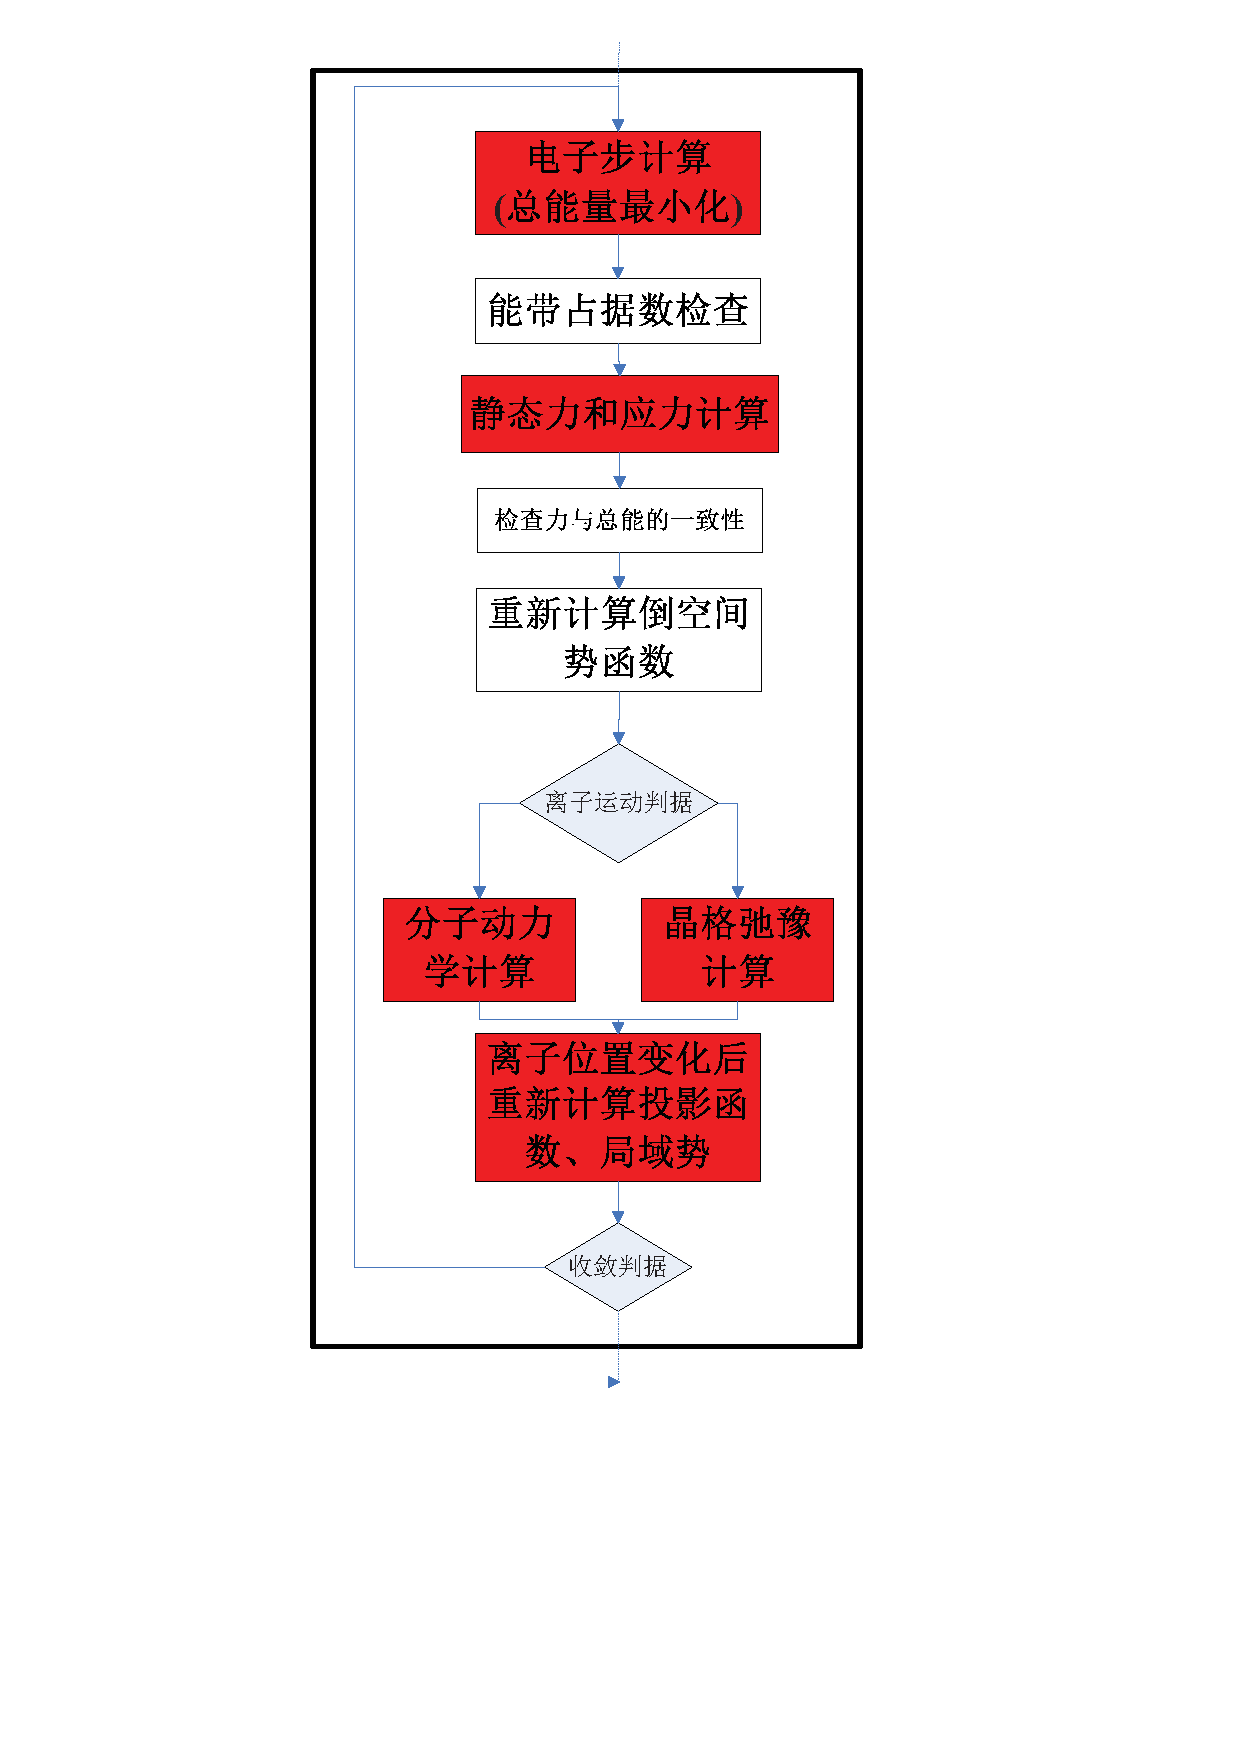
\includegraphics[height=3.72in,width=2.5in,viewport=146 173 436 812,clip]{Figures/VASP_main_Flow-3.pdf}
\caption{\small \textrm{Calculation of the K-S ground-states.}}%
\label{VASP_Follow-3}
\end{figure}
}

\frame
{
\frametitle{}
\begin{figure}[h!]
\centering
\vspace*{-0.80in}
%\hspace*{-10pt}
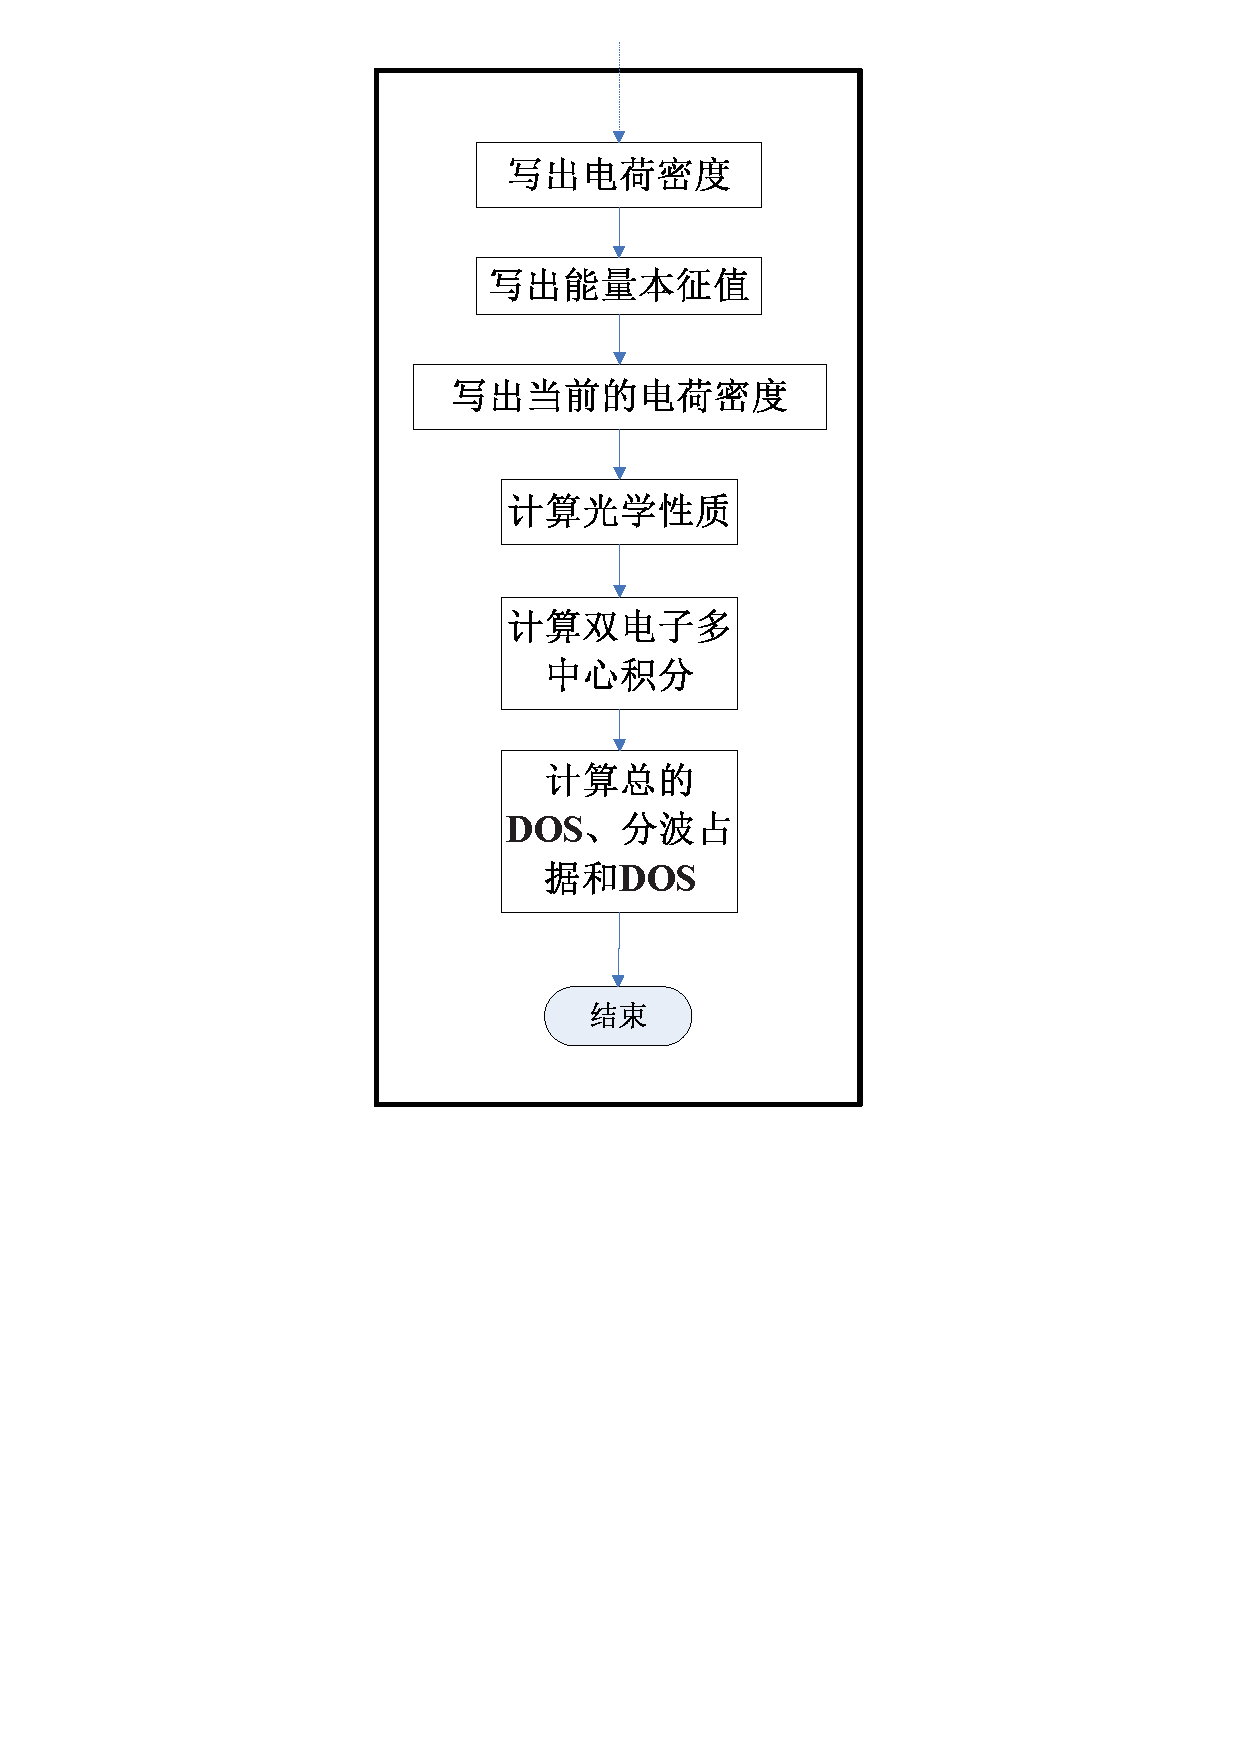
\includegraphics[height=3.70in,width=2.5in,viewport=170 300 417 813,clip]{Figures/VASP_main_Flow-4.pdf}
\caption{\small \textrm{Calculation of the K-S ground-states.}}%
\label{VASP_Follow-4}
\end{figure}
}

%-------------------------------------------------------------------------Thanks------------------------------------------------------------------------------------------------
%\section{致谢}
%\frame
%{
%\frametitle{致$\quad$谢}
%\begin{itemize}
%    \setlength{\itemsep}{20pt}
%  \item 感谢本团队高兴誉、吴泉生、宋红州等各位老师参与的讨论
%  \item 感谢莫所长、宋主任以及软件中心各位老师和同事
%  \item 感谢王崇愚先生的帮助
%\end{itemize}
%}

\logo{}									%不显示logo
\frame
{
\vskip 60 pt
%\hskip 10pt \textcolor{blue}{\Huge 感谢答辩委员会各位老师\,\textrm{!}}\\
\vskip 35 pt
\hskip 60pt \textcolor{blue}{\Huge 谢谢大家\:!}
%\vskip 15 pt
%\hskip 40pt \textcolor{blue}{\Huge \textrm{for your attention\:!}}
}

%-------------------------------------------------------------------------------------------------------------------------------------------------------------------------------

\clearpage
%\end{CJK*}
\end{document}
